\documentclass[11pt]{article}

% arXiv: any class compilable with pdflatex is accepted; no template required.
\usepackage[margin=1in]{geometry}
\usepackage{graphicx}
\usepackage{booktabs}
\usepackage{amsmath}
\usepackage{amssymb}
\usepackage[numbers,sort&compress]{natbib}
\usepackage{caption}
\usepackage{tikz}
\usetikzlibrary{arrows.meta,positioning,fit,backgrounds,calc}
\usepackage[hidelinks]{hyperref}

\captionsetup{font=small,labelfont=bf}
\setlength{\abovecaptionskip}{6pt}
\setlength{\belowcaptionskip}{2pt}

\newcommand{\arm}[1]{\textsc{#1}}
\newcommand{\ctx}{\textsc{ctx}}

\title{\bfseries Reranker-Free Edge Retrieval:\\
Distilling Contextual Chunk Enrichment into a 0.6B Model}

\author{Egor Surovtsev}

\date{}

\begin{document}

\maketitle

\begin{abstract}
Contextual retrieval prepends a short document-level summary to every chunk
before indexing, and the published recipe pairs it with a cross-encoder reranker
to restore the precision that flat chunks lose. Neither stage is cheap outside a
datacenter, and this paper asks whether an edge pipeline needs both. We label
3{,}134 chunks from 82 Russian business documents with an API teacher (24.3M
prompt tokens, USD~0.82) and distill the teacher's contextual enrichment into
\texttt{Qwen3-0.6B} with LoRA. Retrieval is then measured with
\texttt{Qwen3-Embedding-0.6B}, BM25, reciprocal rank fusion and
\texttt{Qwen3-Reranker-0.6B} on an Apple~M2 GPU (MLX, fp16): six configurations
on 234 synthetic queries that carry gold chunks, and all eight on a stratified
subset of sixty. On that subset a reranker-free pipeline with distilled
on-device context reaches 0.600 recall@10 against 0.650 for the same index with
a 0.6B cross-encoder, a difference whose paired bootstrap interval includes
zero, at a median latency of 41.4~ms against 54.7~s, a factor of 1{,}322, while
reranking flat chunks is dominated by the contextual dense-only arm. On this
homogeneous corpus BM25 fusion degrades quality and no setting of the fusion
parameters recovers the loss. Distilling the context generator costs little in
quality: the student lands within 0.04 recall@10 of the teacher while improving
recall@1 and MRR, and with Matryoshka truncation to 512 dimensions plus a
Russian query instruction it matches the teacher baseline on recall@1 and MRR at
half the index size. Generating the contexts for the whole corpus takes 1.85~h
and USD~0.82 through the API, or 4.49~h at no cost on the device, where no
document leaves the machine. The dataset, the adapter, the evaluation harness
and the measurement scripts are released (Section~\ref{sec:availability}).

\end{abstract}

\section{Introduction}
\label{sec:intro}

Retrieval-augmented generation is only as good as the passages it retrieves,
and a chunk that has been cut out of its document frequently reads as
ambiguous on its own. Contextual retrieval attacks this at indexing time by
prepending to each chunk a short summary of the document it came from, which
measurably reduces retrieval failures \citep{anthropic2024contextual}. The
published recipe does not stop there: it also reranks the fused candidate list
with a cross-encoder.

Neither stage is cheap once the system leaves a datacenter. Enrichment costs a
language-model call per chunk, though this is paid once, at ingest, and can be
amortized over many queries. The reranker is paid on every query, one forward
pass per candidate, and on a laptop or a phone that is the cost that hurts:
sixty-four candidates through a 0.6B cross-encoder take tens of seconds, while
a dense-only first stage answers in tens of milliseconds. If the contextual
enrichment has already resolved the ambiguity the reranker was meant to fix,
the reranker can be dropped, and the whole pipeline becomes usable
interactively on a single device. This paper takes up that possibility and
tests it on a corpus of the kind an edge deployment actually meets.

Three questions organize the study. Is a reranker still needed once chunks are
contextualized? Can the enrichment itself be moved on-device, by distilling an
API teacher into a small local model, without giving up retrieval quality? And
which parts of the standard recipe, BM25 fusion, embedding dimension and the
language of the query instruction among them, actually help on a small,
homogeneous, non-English corpus? Published results report the recipe's two
components together, so the three questions cannot be answered from them
directly.

The corpus is 82 Russian business documents that came out of our own OCR
pipeline. It is deliberately small and stylistically uniform: a few hundred
documents that share vocabulary, layout and boilerplate, which is the setting an
edge deployment faces. Every one of the 3{,}134 chunks is labeled by an API
teacher, a 0.6B student is trained to reproduce the teacher's contexts, and
retrieval is evaluated with a purpose-built set of 234 queries carrying gold
chunks. All measurements are taken on a single Apple~M2 with MLX in fp16, the
same machine that would serve the queries.

Our contributions are the following.

\begin{enumerate}
  \item A contextual chunk dataset of 3{,}134 labeled chunks over 82 Russian
  documents, with category and table metadata, produced by an API
  teacher for USD~0.82 and released publicly (\S\ref{sec:data}).
  \item A 0.6B LoRA student that reproduces the teacher's contexts (word-level
  F1 improves from 0.189 to 0.537) and can regenerate the entire corpus
  on-device in 4.49~h at zero marginal cost (\S\ref{sec:distill}).
  \item An eight-arm retrieval evaluation, six configurations on 234 gold-chunk
  queries and all eight on a common stratified subset of sixty, showing that a
  reranker-free pipeline with distilled on-device context comes within 0.05
  recall@10 of the same index with a 0.6B cross-encoder at a factor of 1{,}322
  in median latency, and that reranking flat chunks is dominated by the
  contextual dense-only arm (\S\ref{sec:results-main}).
  \item A negative result for lexical fusion: on this homogeneous corpus BM25
  degrades every configuration, and neither the fusion weights, the rank
  constant nor the retrieval depth recover the loss (\S\ref{sec:ablations}).
  \item Two cheap levers for the on-device path, Matryoshka truncation to 512
  dimensions and a Russian query instruction, that together lift the student
  pipeline to the teacher baseline at half the index size
  (\S\ref{sec:ablations}).
  \item A stratified analysis of where distillation transfers and where it does
  not, and a break-even model that separates ingest cost from query cost
  (\S\ref{sec:strata}, \S\ref{sec:breakeven}).
\end{enumerate}

\section{Related Work}
\label{sec:related}

\paragraph{Chunk enrichment.}
Retrieval quality is decided as much by what is indexed as by the encoder.
Document expansion by query prediction appends generated queries to a passage
before indexing \citep{nogueira2019document}, and proposition-level indexing
replaces passages with self-contained statements
\citep{chen2024densex}. A recent taxonomy and evaluation of chunking strategies
shows that the choice of chunking policy interacts strongly with the retriever
\citep{zhou2026chunking}, while late chunking embeds a whole document before
splitting it, so that every chunk vector already carries document context
\citep{mortezaagha2026latechunking}. Contextual retrieval works along the same
lines, with a document-conditioned summary prepended to each chunk
\citep{anthropic2024contextual}. These methods are usually evaluated together
with a cross-encoder reranker, and the published recipe reports the two
components jointly, which makes their individual contributions hard to
disentangle. We hold first-stage retrieval fixed and vary only the index text and the
presence of the reranker, and we go one step further by distilling the
enrichment model itself so that the ingest stage also runs on-device.

\paragraph{Reranking and late interaction.}
Cross-encoder reranking is an established second stage over a first-stage
candidate list \citep{nogueira2019passage}, and late-interaction models such as
ColBERT retain token-level matching without a full cross-encoder
\citep{khattab2020colbert}. A controlled study of long-context question
answering finds that learned context planning and reranking do not improve over
strong first-stage retrieval \citep{li2026reranking}, which agrees with our
negative result. Modern instruction-tuned embedders and rerankers supply both
stages from a single model family \citep{qwen3embedding}. Reranking is usually
reported as effective, but it scales linearly in the candidate pool and is the
most expensive part of an interactive pipeline on a laptop. We quantify that
cost on a fixed device, and find that once the chunks are contextualized the
reranker can be dropped with no measurable loss in quality.

\paragraph{Hybrid retrieval and fusion.}
Sparse lexical retrieval with BM25 remains a strong baseline
\citep{robertson2009bm25}, and learned sparse models such as SPLADE improve on
it \citep{formal2021splade}. Dense and sparse lists are commonly combined with
reciprocal rank fusion \citep{cormack2009reciprocal}, and self-contained
tooling for hybrid retrieval over quantized embeddings and lexical indexes is
available \citep{livieris2026quanta}. Hybrid retrieval is reported to help on
heterogeneous corpora \citep{luan2021sparse}, but the benefit depends on how
much the two channels complement each other. Our corpus is homogeneous, and we
find that fusion hurts consistently, including with a stronger sparse backend.

\paragraph{Distillation and parameter-efficient tuning.}
Knowledge distillation transfers the behavior of a large model to a smaller
one \citep{hinton2015distilling}, and low-rank adaptation makes the transfer
cheap \citep{hu2022lora,dettmers2023qlora}. We use LoRA over a 4-bit base model
to distill an API teacher into 0.6B parameters, and we judge the student by the
retrieval quality it supports rather than by generation quality alone.
Distilling a retrieval-augmented pipeline for smartphone deployment has been
studied in the legal domain \citep{kamal2026smartphone}, and on-premise
deployments select sub-networks that fit the local hardware
\citep{rizeakos2026onprem}.

\paragraph{Efficient retrieval on device.}
Matryoshka representation learning trains embeddings whose prefixes are
individually usable, which allows truncation with little loss
\citep{kusupati2022matryoshka}; dimension-elastic indexes serve several
truncation levels from one resident index \citep{culatana2026mrvq}, and
sentence encoders provide the dense backbone
\citep{reimers2019sentence,karpukhin2020dense}. Retrieval-augmented generation
\citep{lewis2020retrieval} and its surveys \citep{gao2023retrieval} describe
the full pipeline; the practical constraint in our setting is that every
component must fit and run on one consumer device. We therefore report latency
and cost alongside quality, and we build on the MLX framework for Apple silicon
\citep{mlx} with a local vector index \citep{qdrant}.


\section{Data}
\label{sec:data}

\subsection{Corpus and chunking}

The corpus consists of 82 Russian business documents: construction estimates
and specifications, food-supply invoices and menus, IT contracts, pharmacy
price lists and security policies. Text is obtained with an OCR pipeline
(\texttt{Tesseract} and a lightweight \texttt{PP-OCR} variant as a fallback
\citep{smith2007tesseract,du2020ppocr}), normalized, and split into windows of
at most 8{,}000 tokens at paragraph boundaries. Within a window, text is
further split into chunks of at most 1{,}200 tokens, with tables handled
separately: a table is emitted as a single chunk of at most 1{,}500 tokens and
eight rows, so that headers and their values stay together. Chunks are
contiguous segments of a window, so adjacent chunks share vocabulary; the
median word-level Jaccard similarity of neighboring chunks is 0.31. This
matters at evaluation time, since a retrieved neighbor is frequently a valid
answer (Section~\ref{sec:queries}).

Every chunk is described by metadata: document identifier, category, chunk
index within the document, table flag, token counts, and a content hash of its
window. Near-duplicate documents and duplicate
(window,~chunk) pairs are removed before labeling; the window hash is later
used as the grouping key for the train/validation split, so that no window
appears on both sides.

\subsection{Context labelling}

Each chunk is labeled by an API teacher
(\texttt{deepseek-v4.1-flash}, reasoning disabled). The prompt contains the
full document window and the chunk, and asks for a short context that situates
the chunk within the document and resolves pronouns, abbreviations and table
headers. Prompt caching is effective here, since all chunks of a window share the
same prefix: the overall cache hit rate is 79.3\%, which brings the cost of
labeling the whole corpus down to USD~0.82.

The prompt explicitly forbids adding facts that are absent from the document,
and the audit checks this. Table~\ref{tab:dataset} summarizes the resulting
dataset. The median chunk is 461 tokens long, while the median generated
context is only 296 characters, so the enrichment is cheap to store.

\begin{table}[t]
\centering
\small
\caption{Dataset statistics. Chunks are segments of overlapping document windows, extracted from 82 Russian business documents. Contexts were labeled by an API teacher (\texttt{deepseek-v4.1-flash}, reasoning off) with 79.3\% prompt-cache hit rate.}
\label{tab:dataset}
\begin{tabular}{lr}
\toprule
Property & Value \\
\midrule
Documents & 82 \\
Chunks (window$\rightarrow$context pairs) & 3134 \\
Median chunk length (tokens) & 461 \\
Median generated context (characters) & 296 \\
Table chunks & 1608 \\
\midrule
\quad construction & 211 \\
\quad food & 496 \\
\quad it & 1879 \\
\quad pharma & 239 \\
\quad security & 309 \\
\midrule
Teacher prompt tokens (total) & 24.31M \\
Teacher labeling cost & \$0.82 \\
\midrule
Train / validation chunks & 2701 / 433 \\
Split unit & \texttt{window\_hash} \\
\bottomrule
\end{tabular}
\end{table}


\subsection{Query set}
\label{sec:queries}

Retrieval is evaluated with 234 queries that carry gold chunks. Candidate
queries are generated by two language models from document windows, paraphrased
and judged by one of the two, filtered automatically for identifier leakage and
trivial overlap, and finally reviewed by hand; 234 of the 276 candidates (85\%)
were accepted, at a cost of USD~0.32. The set covers five categories and four
query types: lexical (62), multi-hop (57), semantic (56) and table-oriented (59).

Because chunks are contiguous segments of overlapping windows, a single
question often has several acceptable answers. The evaluation therefore uses
gold groups: for each query, all chunks with the same document identifier whose
chunk index lies within two positions of the gold chunk, or whose text
overlaps the gold chunk with Jaccard similarity above 0.9, are treated as
correct. Metrics that ignore this grouping underestimate dense retrieval, which
tends to return a neighboring window of the correct text.

A manual spot check of twenty query--chunk pairs found seventeen clearly
correct, two debatable and one mismatch. The query set is synthetic, and we
therefore treat absolute metric values as optimistic by roughly five to fifteen
percent; comparisons between arms are made on the same set and are unaffected
by this bias.

\begin{figure}[t]
\centering
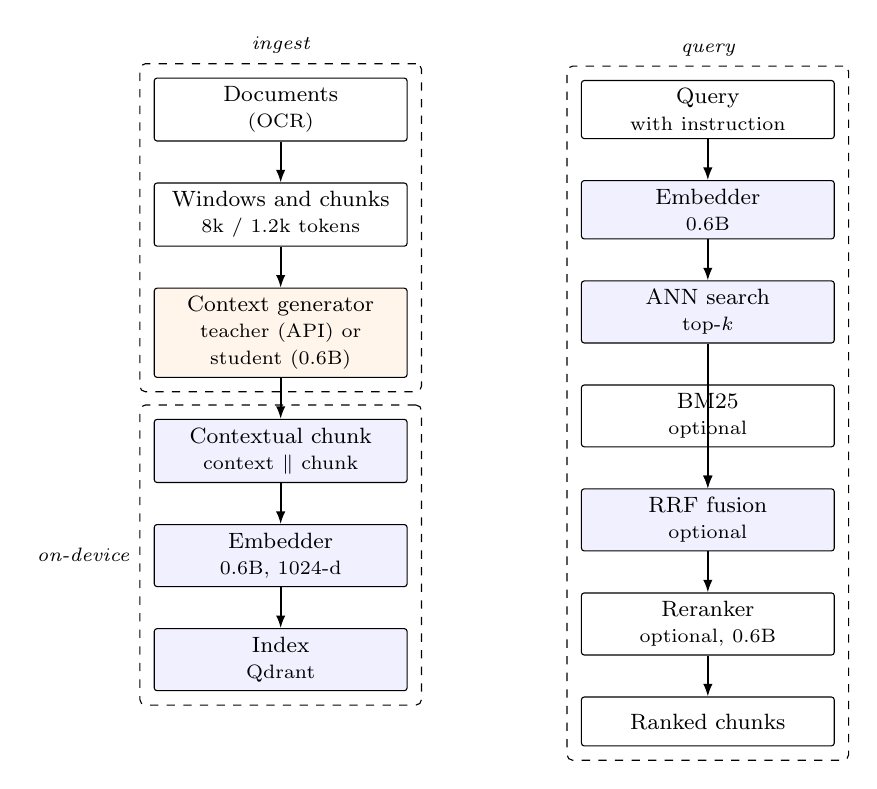
\begin{tikzpicture}[
  font=\footnotesize,
  node distance=5.2mm,
  box/.style={draw, rounded corners=1pt, align=center, inner sep=3pt,
              minimum height=6.2mm, text width=30mm, fill=white},
  dev/.style={box, fill=blue!6},
  api/.style={box, fill=orange!8},
  arr/.style={-{Latex[length=1.6mm]}, semithick},
  phase/.style={draw, dashed, rounded corners=2pt, inner sep=5pt}
]

% ---- left column: ingest
\node[box] (ocr) {Documents\\ \scriptsize (OCR)};
\node[box, below=of ocr] (win) {Windows and chunks\\ \scriptsize 8k / 1.2k tokens};
\node[api, below=of win] (gen) {Context generator\\ \scriptsize teacher (API) or student (0.6B)};
\node[dev, below=of gen] (cc) {Contextual chunk\\ \scriptsize context $\Vert$ chunk};
\node[dev, below=of cc] (emb) {Embedder\\ \scriptsize 0.6B, 1024-d};
\node[dev, below=of emb] (idx) {Index\\ \scriptsize Qdrant};

\draw[arr] (ocr) -- (win);
\draw[arr] (win) -- (gen);
\draw[arr] (gen) -- (cc);
\draw[arr] (cc) -- (emb);
\draw[arr] (emb) -- (idx);

% ---- right column: query
\node[box, right=22mm of ocr] (q) {Query\\ \scriptsize with instruction};
\node[dev, below=of q] (qemb) {Embedder\\ \scriptsize 0.6B};
\node[dev, below=of qemb] (ann) {ANN search\\ \scriptsize top-$k$};
\node[box, below=of ann] (bm) {BM25\\ \scriptsize optional};
\node[dev, below=of bm] (fuse) {RRF fusion\\ \scriptsize optional};
\node[box, below=of fuse] (rer) {Reranker\\ \scriptsize optional, 0.6B};
\node[box, below=of rer] (out) {Ranked chunks};

\draw[arr] (q) -- (qemb);
\draw[arr] (qemb) -- (ann);
\draw[arr] (ann) -- (fuse);
\draw[arr] (bm) -- (fuse);
\draw[arr] (fuse) -- (rer);
\draw[arr] (rer) -- (out);

\begin{scope}[on background layer]
  \node[phase, fit=(ocr) (gen), label={[font=\scriptsize\itshape]above:ingest}] {};
  \node[phase, fit=(cc) (idx), label={[font=\scriptsize\itshape]left:on-device}] {};
  \node[phase, fit=(q) (out), label={[font=\scriptsize\itshape]above:query}] {};
\end{scope}

\end{tikzpicture}
\caption{System overview. Ingest (left) is executed once per document; the
dashed frames separate the API teacher from components that run on the target
device. Query processing (right) is executed per request; BM25 fusion and the
reranker are the two optional stages evaluated in Section~\ref{sec:results}.
Without the two optional stages a query takes about 40~ms at the median.}
\label{fig:pipeline}
\end{figure}

\section{Distilling the Context Generator}
\label{sec:distill}

The teacher produces high-quality contexts but requires an API call per chunk
and sends document text to a third party. We therefore distill the teacher into
\texttt{Qwen3-0.6B} \citep{qwen3} so that the ingest stage runs locally.

\paragraph{Training.}
The student is fine-tuned with QLoRA \citep{dettmers2023qlora}: the base model
is loaded in 4-bit precision, and low-rank adapters \citep{hu2022lora} with
rank 16 and scaling factor 16 are attached to all linear layers, which
corresponds to 1.665\% of the parameters (10.1M of 606.1M). Training uses two
epochs with an effective batch size of eight, a learning rate of
$2\times10^{-4}$, and a maximum sequence length of 16{,}384 tokens; the longest
training sample is 9.7k tokens, so no sample is truncated. Loss is computed on
the assistant response only, with the document and the instruction masked out.
The training and inference prompts are byte-identical
chat templates with thinking disabled, which is enforced by a hard check before
training.

\paragraph{Quality.}
Table~\ref{tab:distill} compares the base model and the fine-tuned student on
sixty held-out chunks, using word-level F1 against the teacher context as the
metric. The base model is unusable: it produces empty or unrelated output, with
a mean F1 of 0.189 and 1.7\% empty responses. After fine-tuning, the mean F1 is
0.537, the tenth percentile rises from 0.064 to 0.319, and no response is
empty. Neither model emits numbers that are absent from the source document, so
the improvement does not come from hallucinated detail. Generation is slightly
slower per sample (7.82~s against 5.55~s) because the fine-tuned model produces
longer, more specific contexts instead of short generic ones.

\begin{table}[t]
\centering
\small
\caption{Distillation quality: word-level F1 of generated contexts against the teacher, on 60 held-out chunks (base Qwen3-0.6B vs.\ the same model after LoRA SFT).}
\label{tab:distill}
\begin{tabular}{lrr}
\toprule
Metric & Baseline & After SFT \\
\midrule
word-F1 mean & 0.189 & \textbf{0.537} \\
word-F1 median & 0.176 & 0.534 \\
word-F1 p10 & 0.064 & 0.319 \\
Empty responses & 1.7\% & \textbf{0\%} \\
Hallucinated numbers & 0 & 0 \\
Generation time / sample (s) & 5.55 & 7.82 \\
\bottomrule
\end{tabular}
\end{table}


\paragraph{Corpus-wide ingest.}
We regenerate the context for all 3{,}134 chunks with the student on the target
device (Apple~M2, MLX in bfloat16). All chunks of a window share the same
prefix, so its key/value state is computed once and reused, which reduces
prefill from an estimated 7.08~h to 2.31~h, a factor of 3.1. Total wall-clock
time is 4.49~h, split into 2.31~h of prefill and 2.19~h of decode; the median
chunk takes 4.20~s. Eleven contexts (0.35\%) reach the 160-token output cap.
The teacher required 1.85~h and USD~0.82, so the on-device path is 2.4 times
slower, costs nothing per run, and never transmits document text.
Table~\ref{tab:ingest} reports the comparison.

\section{Retrieval Harness}
\label{sec:harness}

\paragraph{Device and runtime.}
All measurements are taken on an Apple~M2 (Mac14,2, 8-core GPU) with MLX
\citep{mlx}; the retrieval models run in fp16, while the ingest model of
Section~\ref{sec:distill} runs in bfloat16. The vector index is a local Qdrant
instance without a server process \citep{qdrant}; it stores 3{,}134 points with
fp32 vectors.

\paragraph{Models.}
Dense retrieval uses \texttt{Qwen3-Embedding-0.6B} with 1{,}024-dimensional
output and a maximum input length of 2{,}048 tokens, with the model's query
instruction prepended to each query \citep{qwen3embedding}. Reranking uses
\texttt{Qwen3-Reranker-0.6B} from the same family. Candidates are length-bucketed
and scored in batches of up to sixteen pairs, and the reranker sustains about
1.2 pairs per second end to end at the actual chunk lengths.

\paragraph{Sparse channel and fusion.}
The default sparse channel is an in-memory BM25Okapi implementation with a
Russian Snowball stemmer \citep{robertson2009bm25,porter1980algorithm} and
corpus-calibrated average length. We additionally evaluate the
\texttt{Qdrant/bm25} sparse backend, which applies IDF on the server side; the
backend is eighteen stop-word files and a Python implementation, with no neural
network involved. Dense and sparse lists are combined with reciprocal rank fusion
\citep{cormack2009reciprocal} with the rank constant fixed at $k=60$.

\paragraph{Metrics.}
We report recall at 1, 5, 10 and 50, MRR@10, nDCG@10, document-level recall@10
and the fraction of queries for which the gold group is absent from the top 50
(\emph{miss@50}); recall@$k$ appears as R@$k$ in the tables. All metrics use the
gold groups of Section~\ref{sec:queries}. Differences between arms are reported
with paired bootstrap intervals over queries (20{,}000 resamples, fixed seed).
Latency is measured per query after warm-up and reported as the median and the
95th percentile over the evaluated query set; arms \arm{c} and \arm{d} are timed
on the sixty-query subset of Section~\ref{sec:results-main}.

\paragraph{Arms.}
Table~\ref{tab:arms} lists the eight configurations. Four of them form a
$2\times2$ design over the index content (flat chunk or contextualized chunk)
and the presence of the reranker; the remaining four isolate dense-only
retrieval and the distilled context. The two indexes differ only in the text
that is embedded, so a difference between arm~\arm{a} and arm~\arm{b} is
attributable to the context alone.

\begin{table}[t]
\centering
\small
\caption{Retrieval arms. \emph{Index text} is what the embedder sees;
\emph{query path} is what happens after the first stage. Arms \arm{c} and
\arm{d} rerank a pool of sixty-four candidates with a 0.6B cross-encoder.}
\label{tab:arms}
\begin{tabular}{lll}
\toprule
Arm & Index text & Query path \\
\midrule
\arm{a} & flat chunk & dense, BM25, RRF \\
\arm{b} & context $\Vert$ chunk & dense, BM25, RRF \\
\arm{c} & context $\Vert$ chunk & dense, BM25, RRF, reranked \\
\arm{d} & flat chunk & dense, BM25, RRF, reranked \\
\arm{e} & flat chunk & dense only \\
\arm{f} & context $\Vert$ chunk & dense only \\
\arm{g} & distilled context $\Vert$ chunk & dense only \\
\arm{h} & distilled context $\Vert$ chunk & dense, BM25, RRF \\
\bottomrule
\end{tabular}
\end{table}

\section{Results}
\label{sec:results}

\subsection{Contextual chunks versus reranking}
\label{sec:results-main}

Table~\ref{tab:retrieval} reports retrieval quality on the full set of 234
queries. Replacing flat chunks with contextualized chunks lifts recall@10 from
0.466 to 0.530 with BM25 fusion (arms \arm{a} and \arm{b}) and from 0.517 to
0.658 without it (arms \arm{e} and \arm{f}). The gain is wider on the dense-only
path, and arm~\arm{f} is the strongest configuration in the table on recall@10,
recall@50, document recall@10 and miss@50.

\begin{table}[t]
\centering
\small
\caption{Retrieval quality on the full set of 234 queries with gold chunks (3{,}134-chunk corpus, Apple~M2, MLX fp16). Metrics use gold groups: a hit on an overlapping neighboring window (within two positions) counts as the same text.}
\label{tab:retrieval}
\footnotesize
\begin{tabular}{lrrrrrrrr}
\toprule
Arm & R@1 & R@5 & R@10 & R@50 & MRR@10 & nDCG@10 & docR@10 & miss@50 \\
\midrule
A: flat, RRF & 0.107 & 0.333 & 0.466 & 0.752 & 0.207 & 0.268 & 0.568 & 0.248 \\
B: contextualized, RRF & 0.192 & 0.423 & 0.530 & 0.859 & 0.288 & 0.345 & 0.615 & 0.141 \\
E: flat, dense-only & 0.141 & 0.410 & 0.517 & 0.821 & 0.259 & 0.321 & 0.650 & 0.179 \\
\textbf{F: contextualized, dense-only} & 0.197 & 0.526 & 0.658 & 0.910 & 0.328 & 0.406 & 0.739 & 0.090 \\
G: distilled, dense-only & 0.218 & 0.517 & 0.620 & 0.897 & 0.342 & 0.409 & 0.709 & 0.103 \\
H: distilled, RRF & 0.197 & 0.414 & 0.530 & 0.863 & 0.288 & 0.345 & 0.632 & 0.137 \\
\bottomrule
\end{tabular}
\end{table}


A single reranked query costs about a minute, so arms \arm{c} and \arm{d} were
run on a subset of sixty queries. Every remaining arm was rerun on the same
subset, and Table~\ref{tab:rerank-subset} reports the result. The subset is a
fixed-seed random draw stratified by query type: fifteen queries of each type,
covering all five categories (14 IT, 14 security, 13 food, 11 pharmacy, 8
construction). Arm-to-arm comparisons hold, but the absolute values here differ
from the full set, where arms \arm{f} and \arm{g} reach 0.658 and 0.620.

Contextualization is the largest effect in the table, and it survives both
query paths: on the dense-only path recall@10 moves from 0.467 in arm~\arm{e} to
0.550 in arm~\arm{f}, on the fused path from 0.400 in arm~\arm{a} to 0.450 in
arm~\arm{b}, and over the full set the dense-only gain is wider still, from
0.517 to 0.658.

The reranker does improve the contextualized index, by an amount comparable to
contextualization itself, but the gain is not statistically resolved at sixty
queries. Recall@10 rises from 0.550 in arm~\arm{f} to 0.650 in arm~\arm{c}, a
paired difference of 0.100 with a 95\% bootstrap interval of $[0.000, 0.200]$;
against the distilled arm~\arm{g} the same comparison gives 0.050, with an
interval of $[-0.150, 0.050]$ for the difference arm~\arm{g} minus arm~\arm{c}.
Reaching 0.650 costs a median latency of 54{,}732~ms against 40.5~ms, a factor
of 1{,}351 over the contextualized dense-only arm.

Reranking flat chunks, in contrast, buys nothing. Arm~\arm{d} spends
43{,}383~ms per query to reach recall@10 of 0.467, which is exactly the value of
the dense-only flat arm~\arm{e} at 39.0~ms. A reranker can only reorder
candidates that the index already contains, and the missing document context is
not among them.

BM25 fusion contributes nothing on this corpus either. Arm~\arm{h} fuses the
distilled context with BM25 and reaches 0.450, the same value as arm~\arm{b} on
teacher context, so fusion pulls the distilled arm down from 0.600 in
arm~\arm{g} to 0.450 in arm~\arm{h}, a paired difference of 0.150 with a 95\%
interval of $[0.017, 0.283]$. Section~\ref{sec:ablations} shows that this is not
a question of tuning.

\begin{table}[t]
\centering
\small
\caption{All eight arms, measured on the same stratified subset of sixty queries (fifteen of each type, all five categories represented). Arm~\arm{g} reaches recall@10 of 0.600 at a median latency of 41~ms, and the reranked arm~\arm{c} reaches 0.650 at 54.7~s.}
\label{tab:rerank-subset}
\begin{tabular}{lrrrrr}
\toprule
Arm & R@1 & R@5 & R@10 & MRR@10 & nDCG@10 \\
\midrule
A: flat, RRF & 0.100 & 0.250 & 0.400 & 0.171 & 0.223 \\
B: contextualized, RRF & 0.150 & 0.350 & 0.450 & 0.233 & 0.284 \\
E: flat, dense-only & 0.033 & 0.350 & 0.467 & 0.177 & 0.247 \\
F: contextualized, dense-only & 0.167 & 0.433 & 0.550 & 0.265 & 0.332 \\
\textbf{G: distilled, dense-only} & 0.217 & 0.483 & 0.600 & 0.327 & 0.392 \\
H: distilled, RRF & 0.167 & 0.317 & 0.450 & 0.237 & 0.287 \\
C: contextualized, RRF, reranked & 0.183 & 0.517 & 0.650 & 0.339 & 0.414 \\
D: flat, RRF, reranked & 0.133 & 0.383 & 0.467 & 0.238 & 0.293 \\
\bottomrule
\end{tabular}
\end{table}


\begin{figure}[t]
\centering
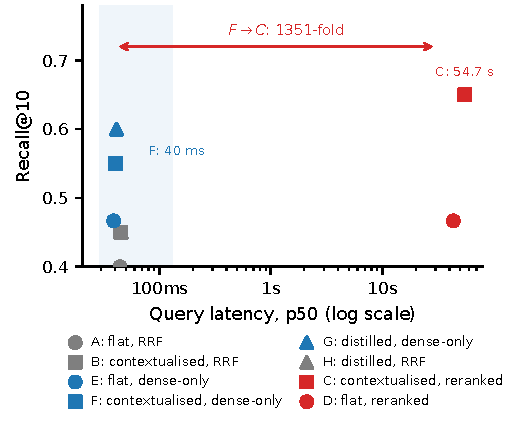
\includegraphics[width=0.62\linewidth]{figures/fig_quality_latency.pdf}
\caption{Quality against median latency, all eight arms on the same sixty
queries (logarithmic horizontal axis). The six reranker-free arms run in tens of
milliseconds; the two reranked arms run for about a minute.}
\label{fig:quality-latency}
\end{figure}

Latency is summarized in Table~\ref{tab:latency}. The reranker-free arms are
hard to tell apart in cost, 39.0 to 45.8~ms per query, of which 32 to 35~ms is
query encoding, while the reranked arms are three orders of magnitude slower. On
a single device that is roughly twenty-five queries per second against one query
per minute.

\begin{table}[t]
\centering
\small
\caption{Query latency (M2 GPU, MLX fp16, warmed). ``Total'' is the end-to-end retrieval call, including query encoding, BM25, fusion and, for arms \arm{c} and \arm{d}, reranking.}
\label{tab:latency}
\begin{tabular}{lrrr}
\toprule
Arm & p50 & p95 & encode \\
\midrule
A: flat, RRF & 44 & 64 & 32 \\
B: contextualized, RRF & 45 & 65 & 32 \\
E: flat, dense-only & 39 & 42 & 34 \\
\textbf{F: contextualized, dense-only} & 40 & 43 & 35 \\
G: distilled, dense-only & 41 & 46 & 35 \\
H: distilled, RRF & 46 & 65 & 32 \\
C: contextualized, RRF, reranked & 54732 & 71445 & 494 \\
D: flat, RRF, reranked & 43383 & 69291 & 365 \\
\bottomrule
\end{tabular}
\end{table}


\subsection{Distilled context on the target device}
\label{sec:results-distill}

Arm~\arm{g} uses contexts generated by the distilled 0.6B student in place of
the API teacher. On the full query set recall@10 falls from 0.658 to 0.620, a
paired difference of 0.038 with a 95\% bootstrap interval of $[-0.021, 0.098]$,
so the two are not distinguishable at this sample size, while MRR@10 and
nDCG@10 rise slightly, from 0.328 to 0.342 and from 0.406 to 0.409. On the
stratified subset the order reverses: the student reaches 0.600 against 0.550
for the teacher, a paired difference of 0.050 with an interval of
$[-0.050, 0.150]$. At this scale the two models are equivalent for retrieval,
and the student needs neither an API key nor a network at ingest time.

The student writes shorter contexts than the teacher, 263 characters against 295
on average, and the stratified analysis of Section~\ref{sec:strata} shows that
the brevity is not uniformly helpful.

Fused with BM25 the student context loses the entire gain: on the stratified
subset arm~\arm{h} reaches 0.450, exactly the value of arm~\arm{b} in the same
flat-versus-contextualized comparison, and on the full set both reach 0.530, so
the distilled context adds nothing once the sparse channel is fused. This is
consistent with the broader observation that the sparse channel is the weaker
component here.

Table~\ref{tab:ingest} gives the ingest comparison. The on-device path takes
4.49~h against 1.85~h for the API, a factor of 2.4, and costs nothing per run;
the prefix key/value cache is what keeps the difference tolerable, since without
it the prefill stage alone would need an estimated 7.08~h.

\begin{table}[t]
\centering
\small
\caption{Context-generation cost for the whole corpus (3{,}134 chunks, 82 documents, 24.3M prompt tokens): API teacher vs.\ distilled 0.6B model running on-device.}
\label{tab:ingest}
\begin{tabular}{lrr}
\toprule
 & Teacher (API) & Student (on-device) \\
\midrule
Model & \texttt{deepseek-v4.1-flash} & \texttt{Qwen3-0.6B} with LoRA \\
Wall-clock (h) & 1.85 & 4.49 \\
Per chunk, median (s) & 2.06 & 4.20 \\
Prefill (h) & -- & 2.31 \\
Decode (h) & -- & 2.19 \\
Output tokens (med./max) & -- & 90/160 \\
Cost (USD) & \textbf{\$0.82} & \textbf{\$0} \\
Data leaves device & yes & no \\
\bottomrule
\end{tabular}
\end{table}


\begin{figure}[t]
\centering
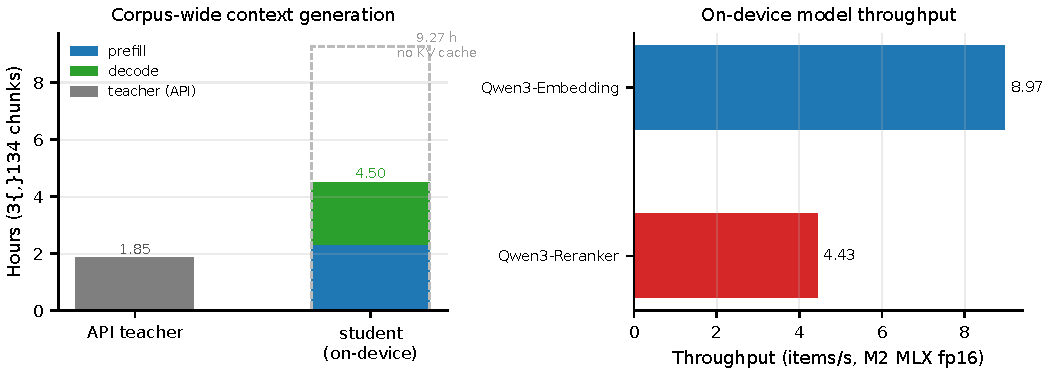
\includegraphics[width=\linewidth]{figures/fig_ingest.pdf}
\caption{Corpus-wide context generation (left) and query-time model throughput
(right). The dashed outline marks the estimated cost of the student without the
prefix key/value cache.}
\label{fig:ingest}
\end{figure}

\subsection{Ablations}
\label{sec:ablations}

Table~\ref{tab:ablations} collects the ablations, computed in memory over the
indexed vectors so that every variant sees identical candidate sets.

\paragraph{Embedding dimension.}
Truncating the 1{,}024-dimensional embeddings to 512 dimensions does not reduce
quality. With teacher context, recall@10 rises from 0.658 to 0.667 and miss@50
falls from 0.090 to 0.064; with student context, recall@10 rises from 0.615 to
0.641 and MRR@10 from 0.341 to 0.354. Truncation to 256 or 128 dimensions
degrades both relative to 512; for the teacher the two values sit close together
(0.568 against 0.573), though we did not run a paired test on those two.

\paragraph{Instruction language.}
Russian works as well as English for the query instruction. On teacher context
it is neutral on recall@10 and slightly better on MRR@10; on student context it
improves recall@10 from 0.615 to 0.650 and MRR@10 from 0.341 to 0.352. The two
levers also combine: truncation to 512 dimensions with a Russian instruction
gives the best student configuration in the table, recall@10 of 0.658 and
MRR@10 of 0.363, which matches the teacher baseline in recall@10 and exceeds it
in MRR@10 at half the vector size.

\paragraph{Fusion.}
No fusion setting recovers the loss caused by the sparse channel. BM25 alone
reaches recall@10 of 0.380 for the teacher context and 0.372 for the student
context, well below the dense-only values of 0.658 and 0.615. Lowering the rank
constant to one, the most favorable setting, still leaves fusion below
dense-only, and raising the weight of the dense channel to a ratio of one to
0.25 approaches but never reaches it. Deepening the BM25 channel from twenty to
two hundred candidates raises teacher recall monotonically from 0.508 to 0.538,
and neither arm reaches the dense-only value.

\begin{table}[t]
\centering
\small
\caption{Retrieval ablations computed in-memory on the indexed vectors (teacher arm F, student arm G; 234 queries, dense-only unless noted). $\Delta$ is student $-$ teacher.}
\label{tab:ablations}
\begin{tabular}{lrrrr}
\toprule
 & \multicolumn{2}{c}{Teacher (F)} & \multicolumn{2}{c}{Student (G)} \\
\cmidrule(lr){2-3}\cmidrule(lr){4-5}
Setting & R@10 & MRR@10 & R@10 & MRR@10 \\
\midrule
\multicolumn{5}{l}{\emph{MRL dimension}} \\
\quad 1024 & 0.658 & 0.328 & 0.615 & 0.341 \\
\quad 512 & 0.667 & 0.328 & 0.641 & 0.354 \\
\quad 256 & 0.568 & 0.303 & 0.611 & 0.332 \\
\quad 128 & 0.573 & 0.296 & 0.586 & 0.302 \\
\addlinespace[2pt]
\multicolumn{5}{l}{\emph{Query instruction}} \\
\quad English & 0.658 & 0.328 & 0.615 & 0.341 \\
\quad Russian & 0.658 & 0.331 & 0.650 & 0.352 \\
\addlinespace[2pt]
\multicolumn{5}{l}{\emph{Hybrid fusion (RRF)}} \\
\quad dense-only & 0.658 & 0.328 & 0.615 & 0.341 \\
\quad BM25-only & 0.380 & 0.189 & 0.372 & 0.184 \\
\quad $k{=}1$, 1:1 & 0.611 & 0.304 & 0.603 & 0.305 \\
\quad $k{=}10$, 1:1 & 0.581 & 0.295 & 0.607 & 0.292 \\
\quad $k{=}60$, 1:1 & 0.530 & 0.289 & 0.517 & 0.266 \\
\quad $k{=}60$, 1:0.25 & 0.645 & 0.314 & 0.603 & 0.297 \\
\addlinespace[2pt]
\multicolumn{5}{l}{\emph{Best combination}} \\
\quad d=512, Russian & 0.675 & 0.331 & 0.658 & 0.363 \\
\addlinespace[2pt]
\bottomrule
\end{tabular}
\end{table}


A stronger sparse backend does not change the picture. Table~\ref{tab:bm25}
compares the in-memory BM25Okapi implementation with the \texttt{Qdrant/bm25}
sparse backend, which applies IDF on the server side. The stronger backend
improves BM25-only recall@10 from 0.325 to 0.355 and hybrid recall@10 from 0.466
to 0.504 for flat chunks and from 0.530 to 0.556 for contextualized chunks, at
about fifty milliseconds per query, but it stays below the dense-only 0.658. On
a homogeneous corpus the sparse channel retrieves documents that share
vocabulary with the query yet do not answer it, and fusion carries that noise
into the dense ranking.

\begin{table}[t]
\centering
\small
\caption{BM25 backend comparison. \texttt{rank\_bm25} is an in-memory BM25Okapi with a Russian Snowball stemmer; \texttt{fastembed} uses \texttt{Qdrant/bm25} sparse vectors with IDF applied server-side (18 stop-word files, 92\,KB, no neural network). Hybrid columns are arms A/B.}
\label{tab:bm25}
\begin{tabular}{lrrrr}
\toprule
Setting & R@10 & MRR@10 & docR@10 & p50 (ms) \\
\midrule
\multicolumn{5}{l}{\emph{BM25-only}} \\
\quad \texttt{rank\_bm25} & 0.325 & 0.136 & 0.414 & 4.1 \\
\quad \texttt{fastembed} & 0.355 & 0.142 & 0.453 & 56.8 \\
\addlinespace[2pt]
\multicolumn{5}{l}{\emph{Hybrid RRF (dense and BM25)}} \\
\quad A flat, \texttt{rank\_bm25} & 0.466 & 0.207 & 0.568 & -- \\
\quad A flat, \texttt{fastembed} & 0.504 & 0.222 & 0.598 & -- \\
\quad B contextualized, \texttt{rank\_bm25} & 0.530 & 0.288 & 0.615 & -- \\
\quad B contextualized, \texttt{fastembed} & 0.556 & 0.286 & 0.645 & -- \\
\bottomrule
\end{tabular}
\end{table}


\subsection{Where distillation transfers}
\label{sec:strata}

Table~\ref{tab:strata} and Figure~\ref{fig:strata} break the teacher and student
arms down by query type, category and the kind of gold chunk.

The student context is the better of the two on multi-hop queries, where
recall@10 rises by 0.018 and MRR@10 by 0.038, and on the food category, where
recall@10 rises by 0.170. Both are settings in which a short context suffices:
multi-hop questions benefit from a concise statement that does not dilute the
connection between distant fragments, and the food documents are the most
template-like in the corpus.

The student is worse on semantic queries, where recall@10 falls by 0.125, and in
the IT, security and pharma categories, where the loss ranges from 0.106 to
0.130. These queries turn on exact details such as numbers, identifiers and
thresholds, and the student tends to generalize. The same pattern shows up in
the gold-chunk breakdown: tables are difficult for both models, with recall@10
between 0.483 and 0.540 against 0.694 to 0.728 on text, and the student loses
more ground on tables than on text.

\begin{table}[t]
\centering
\small
\caption{Per-stratum retrieval quality, teacher context (F) vs.\ student context (G); dense-only, 1024-d, English instruction. $\Delta$ is student $-$ teacher.}
\label{tab:strata}
\begin{tabular}{lrrrr}
\toprule
Stratum & $n$ & F R@10 & G R@10 & $\Delta$ R@10 \\
\midrule
\multicolumn{5}{l}{\emph{Query type}} \\
\quad lexical & 62 & 0.645 & 0.629 & -0.016 \\
\quad multihop & 57 & 0.684 & 0.702 & 0.018 \\
\quad semantic & 56 & 0.714 & 0.589 & -0.125 \\
\quad table & 59 & 0.593 & 0.542 & -0.051 \\
\addlinespace[2pt]
\multicolumn{5}{l}{\emph{Category}} \\
\quad construction & 35 & 0.486 & 0.486 & 0.000 \\
\quad food & 47 & 0.638 & 0.808 & 0.170 \\
\quad it & 59 & 0.712 & 0.593 & -0.119 \\
\quad pharma & 47 & 0.766 & 0.660 & -0.106 \\
\quad security & 46 & 0.630 & 0.500 & -0.130 \\
\addlinespace[2pt]
\multicolumn{5}{l}{\emph{Gold chunk}} \\
\quad gold table & 87 & 0.540 & 0.483 & -0.057 \\
\quad gold text & 147 & 0.728 & 0.694 & -0.034 \\
\addlinespace[2pt]
\bottomrule
\end{tabular}
\end{table}


\begin{figure}[t]
\centering
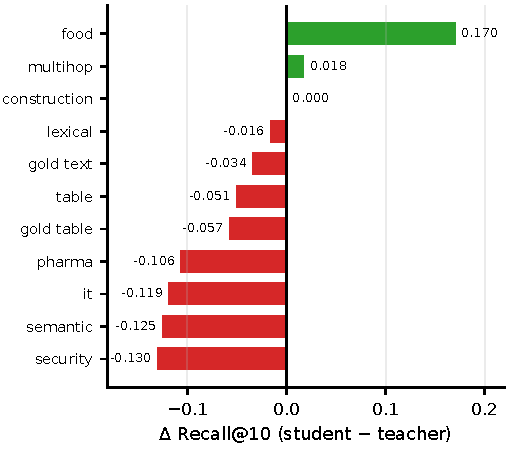
\includegraphics[width=0.60\linewidth]{figures/fig_strata.pdf}
\caption{Change in recall@10 when the teacher context is replaced by the
distilled context, by stratum.}
\label{fig:strata}
\end{figure}

\subsection{Cost and break-even}
\label{sec:breakeven}

The two pipelines differ in where their cost sits. Context generation costs 3.3
minutes per document on the device and 1.4 minutes per document through the API,
and it is paid once per document. Query processing costs 40~ms per query without
the reranker and 54.7~s with it, paid once per query. Writing
$T(D, Q) = D\,t_{\mathrm{ingest}} + Q\,t_{\mathrm{query}}$ for a corpus of $D$
documents and $Q$ queries, the reranker is never worth its query cost at a
practical workload: at $D = 500$ and $Q = 1{,}000$ the on-device reranker-free
pipeline needs 27.4 hours and the API pipeline 11.3 hours for USD~4.98, while
adding the reranker raises these to 42.6 and 26.5 hours respectively.

\begin{figure}[t]
\centering
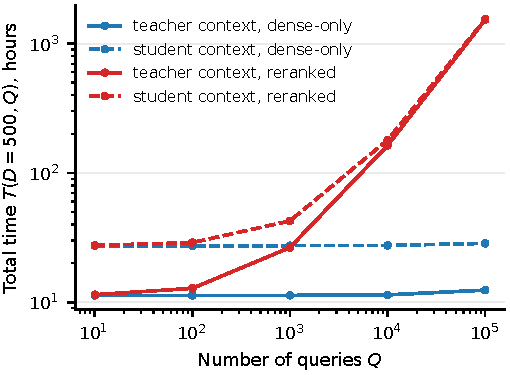
\includegraphics[width=0.62\linewidth]{figures/fig_breakeven.pdf}
\caption{Total time as a function of the number of queries for a corpus of 500
documents. The reranked configurations grow with the query count; the
reranker-free configurations are dominated by ingest.}
\label{fig:breakeven}
\end{figure}

The break-even between the two context generators lies in the ingest cost: the
API saves 2.6 hours per eighty-two documents and costs USD~0.82, while the
on-device path costs nothing and keeps the documents local. The API is
preferable when the corpus is generated once and hardware is the bottleneck;
the on-device path is preferable when the corpus is regenerated, when the
documents are sensitive, or when the device is the only hardware available.

\section{Limitations}
\label{sec:limitations}

\paragraph{Corpus size and homogeneity.}
At 82 documents and 3{,}134 chunks the corpus is a realistic size for an edge
deployment, but far below that of a main-conference retrieval benchmark, so the
results are best read as a case study. The documents themselves are uniform:
they belong to five business categories and share vocabulary, layout and
boilerplate. The negative result for BM25 may well be a property of this
homogeneity, and the size of the recall gains may not transfer either.
Expanding the corpus to several hundred documents is left for future work.

\paragraph{Synthetic queries.}
The query set was generated by two language models, paraphrased and judged by
one of the two, and filtered automatically; a manual spot check of twenty pairs
found seventeen clearly correct, two debatable and one mismatch. Absolute metric
values are therefore optimistic by roughly five to fifteen percent. Every
comparison in this paper is made on the same query set and is unaffected by the
bias, but the values should not be taken as estimates of performance on
naturally occurring questions, since synthetic and authentic query distributions
are known to diverge in ways that aggregate scores do not reveal
\citep{kucia2026synthetic}. Because the judge is also one of the generators, the
acceptance filter shares the generator's blind spots.

\paragraph{Statistical power.}
The reranked arms are measured on sixty queries, which bounds the resolution of
the quality comparison: the bootstrap interval for the gain of the reranker
over the contextualized dense-only arm includes zero
(Section~\ref{sec:results-main}), so this study cannot decide whether a 0.6B
reranker adds quality here. The claim we defend is narrower. The reranker is not
required for the pipeline to work, because the distilled reranker-free
configuration is indistinguishable from the reranked one at three orders of
magnitude lower latency, and because reranking flat chunks does not recover the
missing context. Larger query sets would be needed to resolve what remains.

\paragraph{Ablation methodology.}
The dimension and instruction ablations reuse the indexed 1{,}024-dimensional
vectors and truncate them after the fact. Truncating a Matryoshka embedding is
equivalent to evaluating the corresponding prefix, but a model trained natively
at 512 dimensions could behave differently. The fusion ablations likewise reuse
the dense candidate lists and vary only the fusion parameters.

\paragraph{Reranker configuration.}
The reranked arms use the harness default of sixty-four candidates. An ablation
over pools of 16, 32 and 64 on an earlier sixty-query subset shows identical
recall@10, a small loss in recall@5 at 64, where the reranker begins to reorder
correct pairs, and a latency that is not monotone (42.9~s, 36.6~s and 44.0~s at
pools of 16, 32 and 64). Latency here is dominated by per-call overhead more
than by pool size, so a smaller pool is the better trade at query time, and the
reported arm~\arm{c} and arm~\arm{d} numbers are conservative. We did not
evaluate alternative rerankers; a stronger cross-encoder might change the
quality comparison, though not the latency ratio.

\paragraph{Language and domain.}
The corpus is Russian and the tasks are document-centric. That a Russian query
instruction is at least as good as an English one is specific to this setting,
and it is not a general rule for multilingual retrieval.

\paragraph{No end-to-end evaluation.}
We measure retrieval quality, not answer quality. Word-level F1 against the
teacher context measures how faithfully the student reproduces the teacher, and
the retrieval metrics measure whether the correct chunk is found; neither
measures whether a downstream generator produces a correct answer. A downstream
evaluation could reveal that shorter student contexts are less useful than their
retrieval metrics suggest.

\paragraph{Hardware.}
All measurements come from a single Apple~M2 with MLX, the retrieval models in
fp16 and the ingest model in bfloat16. Absolute latency and throughput will
differ on other devices. The ratio between a 0.6B cross-encoder over a candidate
pool and a single dense search is large enough to hold on any hardware that can
run both, but the exact factor will not.

\section{Conclusion}
\label{sec:conclusion}

We set out to test contextual retrieval on a small, homogeneous, non-English
corpus with a laptop as the deployment target, and arrived at a simpler pipeline
than the published recipe.

What carries the pipeline is the context, not the reranker. On the same sixty
queries, contextualized chunks with dense-only retrieval reach recall@10 of
0.550 in 40.5~ms and the distilled on-device context reaches 0.600 in 41.4~ms,
while the same index behind a 0.6B cross-encoder reaches 0.650 in 54.7~s. The
0.05 gap in recall@10 between the distilled reranker-free arm and the reranked
arm has a paired bootstrap interval that includes zero, which makes the reranker
optional at a factor of 1{,}322 in median latency. Where the index is flat, the
reranker cannot help at all: it spends 43~s per query to return the same recall
as the dense-only flat arm, which answers in 39~ms.

The contextual enrichment itself moves to the target device without much loss.
A 0.6B LoRA student reproduces the teacher's contexts with a mean word-level F1
of 0.537 against 0.189 for the untrained base model, regenerates the whole
corpus in 4.49~h behind a prefix key/value cache, and costs nothing per run.
Retrieval quality is essentially unchanged, and two cheap levers, truncation to
512 dimensions and a Russian query instruction, raise the student pipeline to
the teacher baseline at half the vector size.

Two components of the standard recipe did not survive the move to this corpus.
BM25 fusion degrades every configuration, including with a stronger sparse
backend, and no setting of the fusion parameters recovers the loss; for the
distilled context the drop from 0.600 to 0.450 in recall@10 is the only
difference in this study whose bootstrap interval excludes zero. Distillation is
also uneven across strata: the student beats the teacher on multi-hop queries
and on template-like documents, and trails it on semantic queries and on tables,
which are hard for both models.

The resulting configuration is a single dense index of contextualized chunks,
built once per document on the device that later serves the queries; there are
no API calls at ingest, and no reranker or lexical fusion at query time. On a
laptop GPU it answers roughly twenty-five queries per second.

\subsection{Data and code availability}
\label{sec:availability}

The contextual chunk dataset is available at
\url{https://huggingface.co/datasets/p4ulbr4dl3y/ru-contextual-chunks} and
the distilled model at
\url{https://huggingface.co/p4ulbr4dl3y/qwen3-0.6b-contextual-chunks}. The
retrieval harness, the query set and the scripts that generate every table and
figure in this paper are available at
\url{https://github.com/p4ulbr4dl3y/contextual-chunks}.


\bibliographystyle{plainnat}
\bibliography{refs}

\end{document}
